    %%%%%%%%%%%%%%%%%%%%%%%%%%%%%%%%%%%%%%%%
    %%  Slide 1: <BACKUP>  %%
    %%%%%%%%%%%%%%%%%%%%%%%%%%%%%%%%%%%%%%%%
    \begin{frame}
        Backup        
    \end{frame} 


    %%%%%%%%%%%%%%%%%%%%%%%%%%%%%%%%%%%%%%%%
    %%  Slide 1: <Applications>  %%
    %%%%%%%%%%%%%%%%%%%%%%%%%%%%%%%%%%%%%%%%
    %\begin{frame}
    %    \frametitle{Tracking in HEP}

    %    Task of pixel detectors in tracking:
    %    \begin{itemize}
    %        \item pattern recognition with the identification of particle tracks even in the presence of large backgrounds and pile-up
    %        \item measurement of vertices (primary and secondary)
    %        \item multi-track and vertex separation in the core of jets
    %        \item measurement of specific ionization
    %        \item momentum measurement combining with the information from other detectors
    %    \end{itemize}
    %\end{frame} 


    %%%%%%%%%%%%%%%%%%%%%%%%%%%%%%%%%%%%%%%%
    %%  Slide 1: <>  %%
    %%%%%%%%%%%%%%%%%%%%%%%%%%%%%%%%%%%%%%%%
    \begin{frame}
        \frametitle{}
        \begin{figure}[h!]
            \centering
            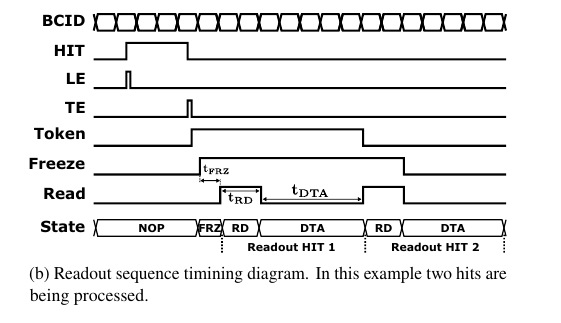
\includegraphics[width=.8\linewidth]{figures/Monopix1/readout_timing.png}
        \end{figure}
    \end{frame} 

    %%%%%%%%%%%%%%%%%%%%%%%%%%%%%%%%%%%%%%%%
    %%  Slide 1: <>  %%
    %%%%%%%%%%%%%%%%%%%%%%%%%%%%%%%%%%%%%%%%
    \begin{frame}
        \frametitle{Radiotherapy}
        \begin{figure}[h!]
            \centering
            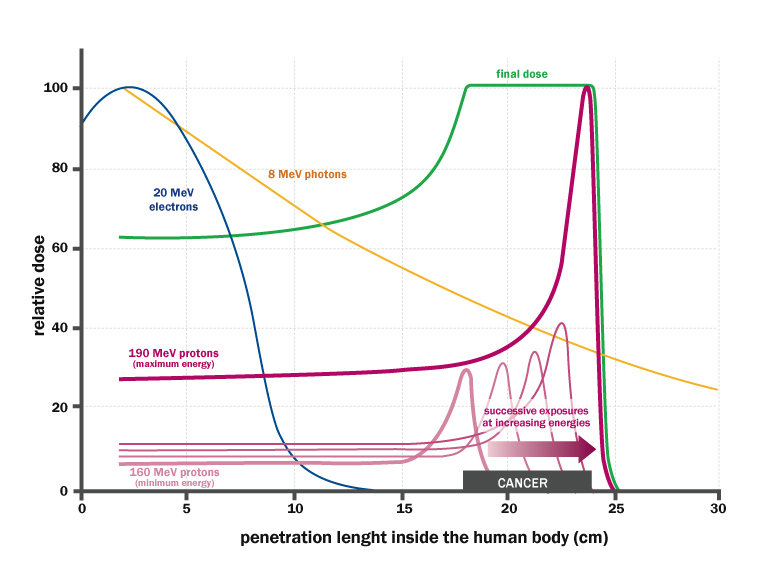
\includegraphics[width=.8\linewidth]{figures/pixel_detectors_usage/Bragg-Peak.png}
        \end{figure}
    \end{frame} 


     %%%%%%%%%%%%%%%%%%%%%%%%%%%%%%%%%%%%%%%%
    %%  Slide 1: <>  %%
    %%%%%%%%%%%%%%%%%%%%%%%%%%%%%%%%%%%%%%%%
    \begin{frame}
        \frametitle{Front end}
            \textbf{ALPIDE like}
            \begin{figure}[h!]
                \centering
                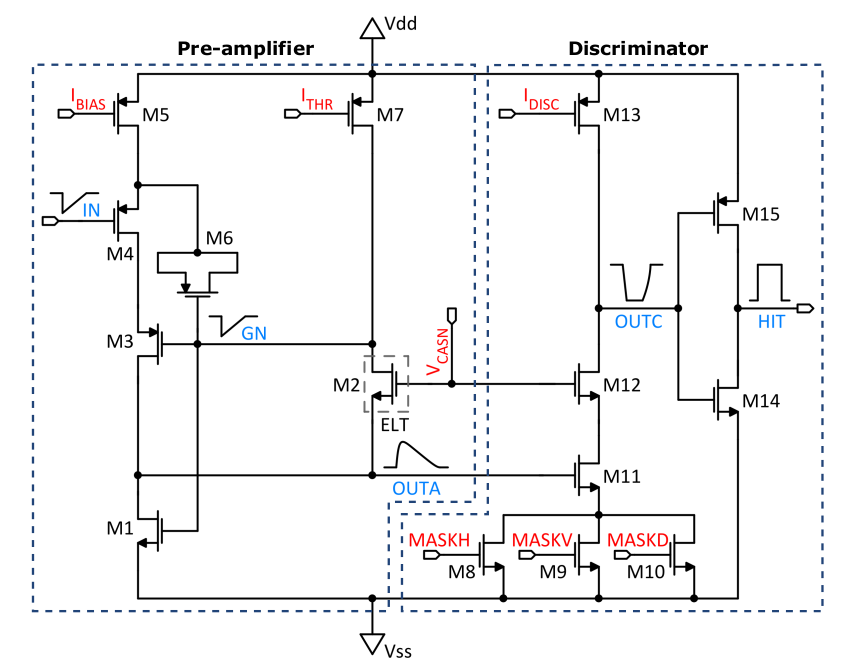
\includegraphics[width=.8\linewidth]{figures/Monopix1/Monopix1_FE_circuit.png}        
            \end{figure}
    \end{frame}     

    
    %%%%%%%%%%%%%%%%%%%%%%%%%%%%%%%%%%%%%%%%
    %%  Slide 3: <Sensors types>  %%
    %%%%%%%%%%%%%%%%%%%%%%%%%%%%%%%%%%%%%%%%
    \begin{frame}
        \frametitle{Sensor types}
            \begin{itemize}
                \item \textbf{Large fill factor} ($\sim$100-200 \si{fF}) or \textbf{small fill factor} ($<$\SI{5}{fF}), depending on the deep p-well structures
            \end{itemize}
            %\centering
            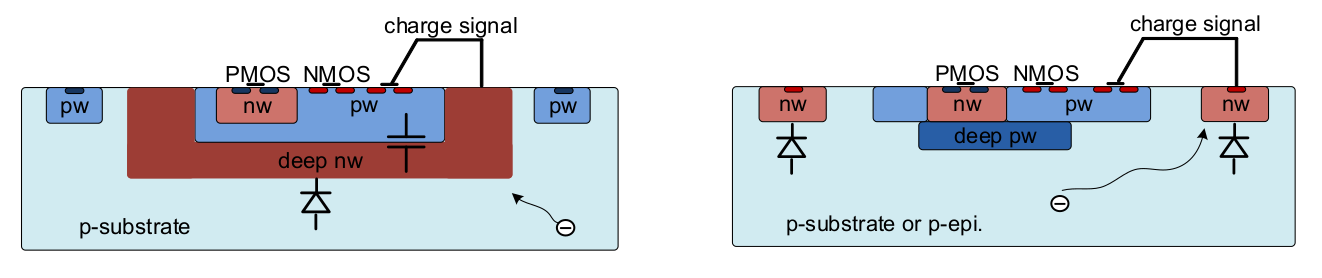
\includegraphics[width=1.05\linewidth]{figures/Pixel_detectors/large_small_sensor_scheme.png}\\
            \begin{columns}
                \column{0.5\textwidth}  
                    %\centering
                    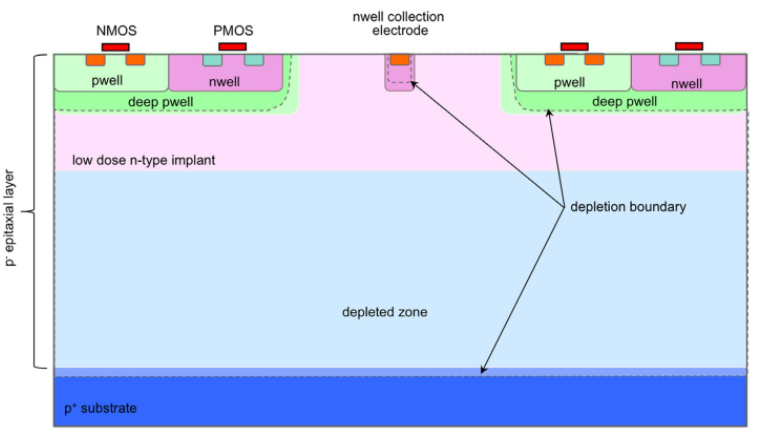
\includegraphics[width=1.1\linewidth]{figures/Pixel_detectors/ALPIDE_after_PM.png}
                \column{0.5\textwidth}  
                    \begin{itemize}
                        \item \textbf{Process modification} with a low dose planar implant. \\
                        whose main investigator is ALICE\\
                        %Advantage: no need of change in the sensor and circuit layout
                    \end{itemize} 
            \end{columns}

            \end{frame} 
    %%%%%%%%%%%%%%%%%%%%%%%%%%%%%%%%%%%%%%%%
    %%  Slide 1: <>  %%
    %%%%%%%%%%%%%%%%%%%%%%%%%%%%%%%%%%%%%%%%
    \begin{frame}
        \frametitle{Noisy pixels}
        \begin{columns}
            \column{0.4\textwidth} 
                \centering
                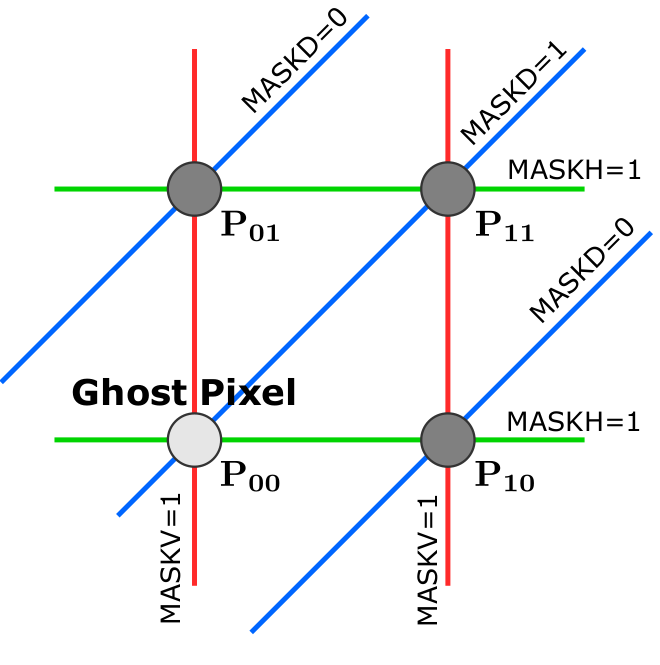
\includegraphics[width=.8\linewidth]{figures/Monopix1/masking_scheme.png}        
            \column{0.4\textwidth} 
            %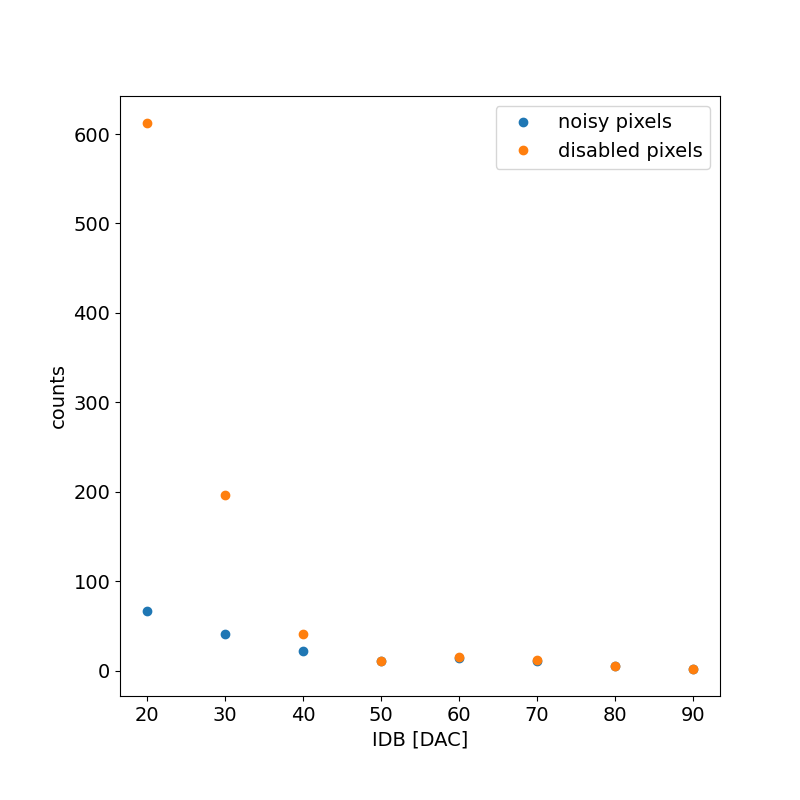
\includegraphics[width=.8\linewidth]{figures/characterization/noisy.png}
        \end{columns}
    \end{frame}    

    %%%%%%%%%%%%%%%%%%%%%%%%%%%%%%%%%%%%%%%%
    %%  Slide 2: <Threshold_noise>  %%
    %%%%%%%%%%%%%%%%%%%%%%%%%%%%%%%%%%%%%%%%
    \begin{frame}
        \frametitle{Threshold and noise results with different FE}
        Noise rate, ma$\sim$\SI{3}{Hz}
        \begin{columns}
            \column{0.45\textwidth}        
                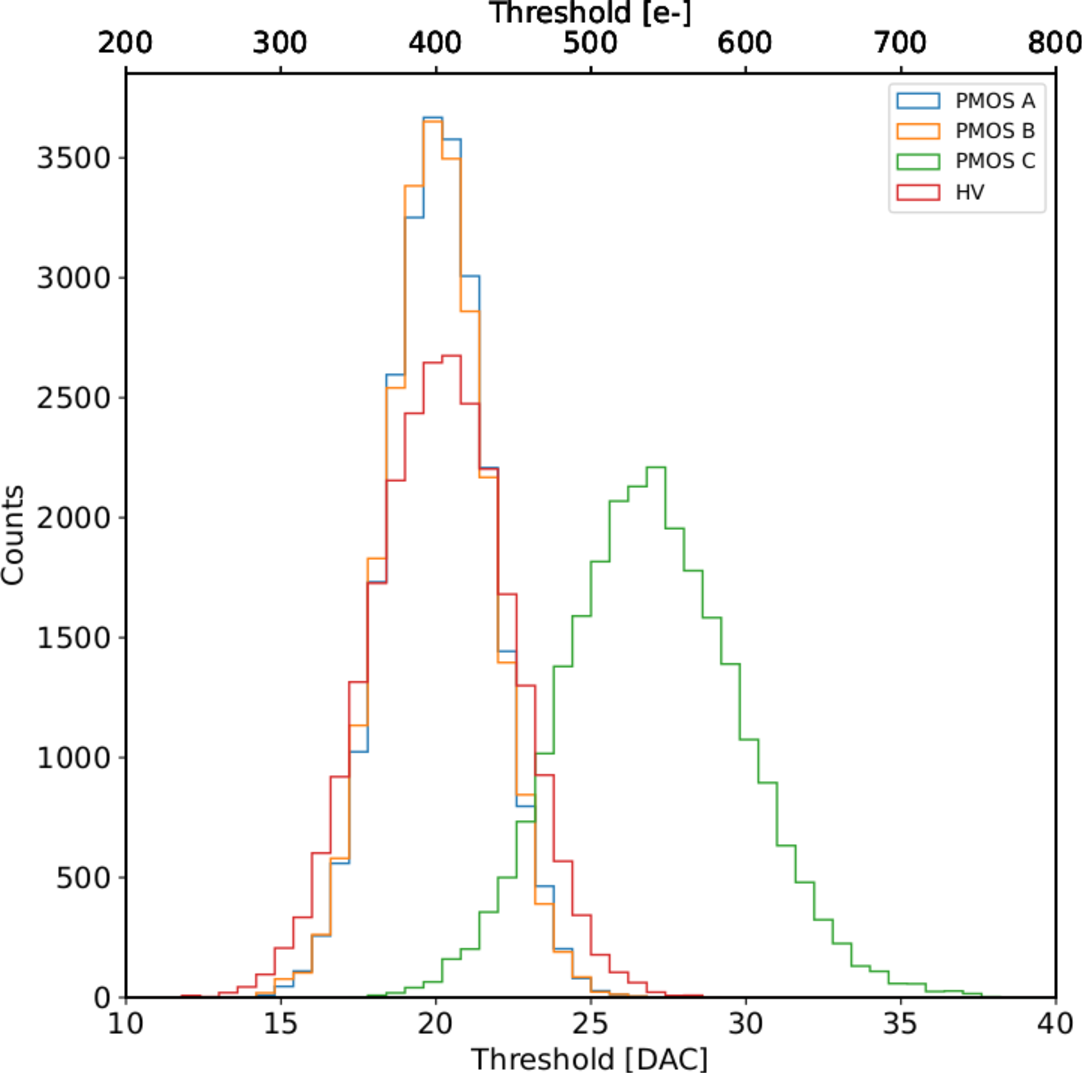
\includegraphics[width=1.1\linewidth]{figures/charaterization/threshold_histogram.pdf}
            \column{0.45\textwidth}        
                \includegraphics[width=1.1\linewidth]{figures/charaterization/noise_histogram.pdf} 
        \end{columns}                  
        \begin{table}[h!]
            \tiny
            \begin{center}
            \begin{tabular}{| c |  c | c | c |c || c|}
            \hline
            & PMOS A & PMOS B & PMOS C & HV & simulation \\
            \hline
            \hline
            Threshold [\si{\elementarycharge}$^-$] & 401.7$\pm$0.2 & 400.8$\pm$0.2 & 539.7$\pm$0.6 &  403.9$\pm$0.2 &\\
            Threshold dispersion [\si{\elementarycharge}$^-$] & 32.9$\pm$0.1 & 33.0$\pm$0.2 & 55.5$\pm$0.4 & 44.7$\pm$0.2 &\\
            Noise [\si{\elementarycharge}$^-$] & 13.01$\pm$0.06 & 12.26$\pm$0.07 & 13.9$\pm$0.1 & 11.7$\pm$0.1 & \\
            Noise dispersion [\si{\elementarycharge}$^-$] & 1.61$\pm$0.04 & 1.50$\pm$0.05 & 1.91$\pm$0.07 & 1.58$\pm$0.07 & \\
            \hline
            \end{tabular}
            \end{center}
        \end{table}       

    \end{frame}

    %%%%%%%%%%%%%%%%%%%%%%%%%%%%%%%%%%%%%%%%
    %%  Slide 1: <MIMOSA>  %%
    %%%%%%%%%%%%%%%%%%%%%%%%%%%%%%%%%%%%%%%%
    \begin{frame}
        \frametitle{MIMOSA series}
        First CMOS MAPS in HEP. Ma aveva rolling shut readout. 
        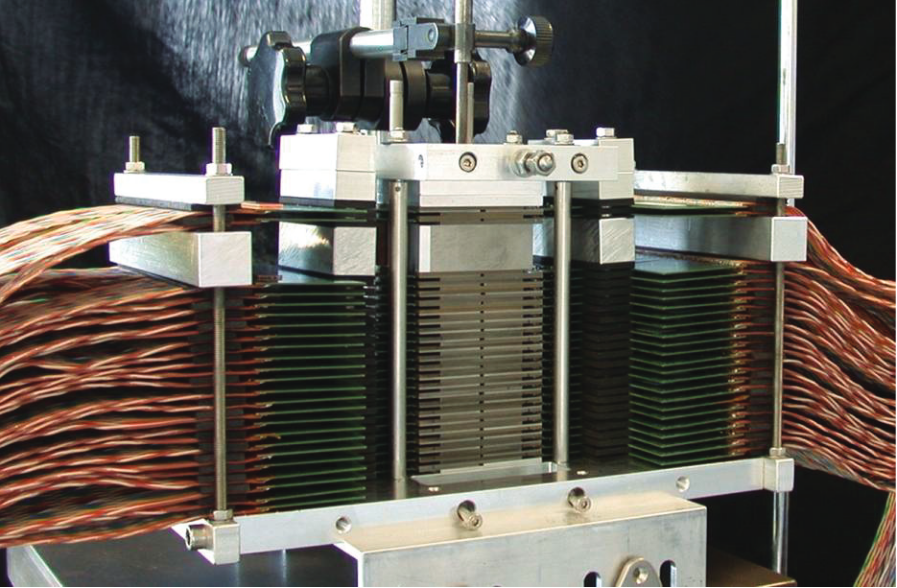
\includegraphics[width=.45\linewidth]{figures/pixel_detectors_usage/ALICE_FoCAL.png} with MIMOSA
    \end{frame} 


    %%%%%%%%%%%%%%%%%%%%%%%%%%%%%%%%%%%%%%%%
    %%  Slide 1: <ALICE>  %%
    %%%%%%%%%%%%%%%%%%%%%%%%%%%%%%%%%%%%%%%%
    \begin{frame}
        \frametitle{ALPIDE - ALice PIxel DEtector}
        ALICE ITS2 upgraded in 2019-20\\
        \smallskip
        The \textbf{sensor} uses high resistivity p-type epi-layer, TowerJazz in \SI{0.18}{\um}. It is the first large area $\sim$\SI{10}{m\squared} MAPS detector with sparsified readout.
        Many MAPS have an \textbf{ALPIDE-based Front End} (i.e. TJ-Monopix1, ARCADIA)
        \begin{columns}
            \column{0.35\textwidth}  
                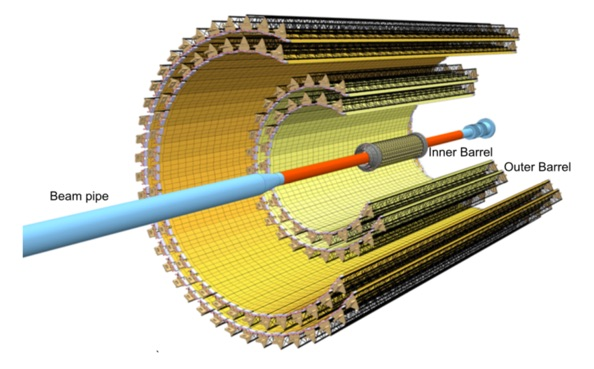
\includegraphics[width=1.3\linewidth]{figures/pixel_detectors_usage/alice.png}
            \column{0.6\textwidth}
            \begin{itemize}
                \item position measurement $\sim$\SI{5}{\um} (pixel dimension 27$\times$29\si{\um\squared})
                \item X$_0$ reduced from 1.14\% to 0.3\% per layer
                \item efficiency of track reconstruction improves of a factor 6 for low momentum particles with $p_T \sim$\SI{0.1}{GeV/c}
            \end{itemize}
        \end{columns}
        %ALPIDE is under test for several other HEP detectors (i.e. Belle2) and applications and 
    \end{frame} 


    %%%%%%%%%%%%%%%%%%%%%%%%%%%%%%%%%%%%
    %% Slide 3: <> %%
    %%%%%%%%%%%%%%%%%%%%%%%%%%%%%%%%%%%%
    \begin{frame}
        \frametitle{Test on beam: preliminary results}
        \begin{itemize}
            \item With \textbf{both} the collimators, DPP=\SI{0.07}{Gy}, t$_p$=\SI{4}{\us}, PRF=\SI{1}{Hz}
        \end{itemize}
        \medskip
        \begin{figure}
            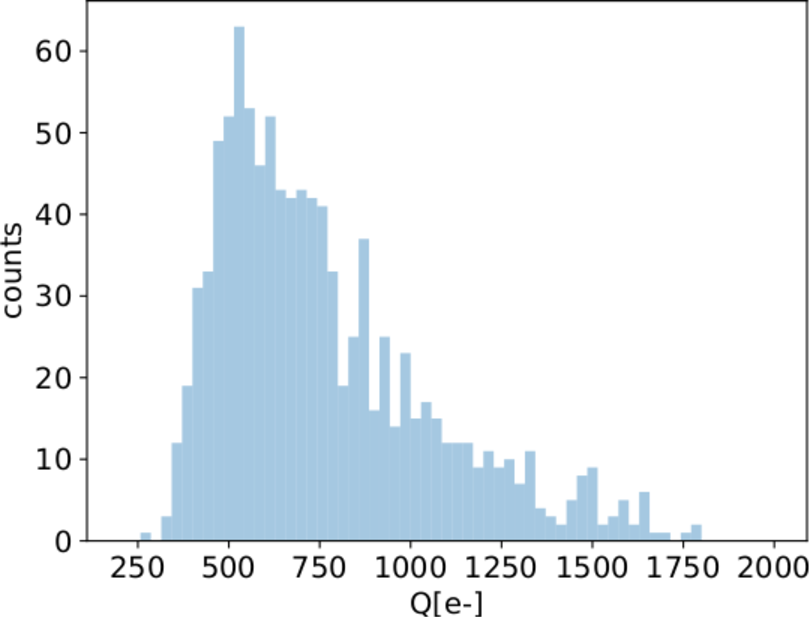
\includegraphics[width=0.49\linewidth]{figures/test_beam/Q1_17_11.pdf}
            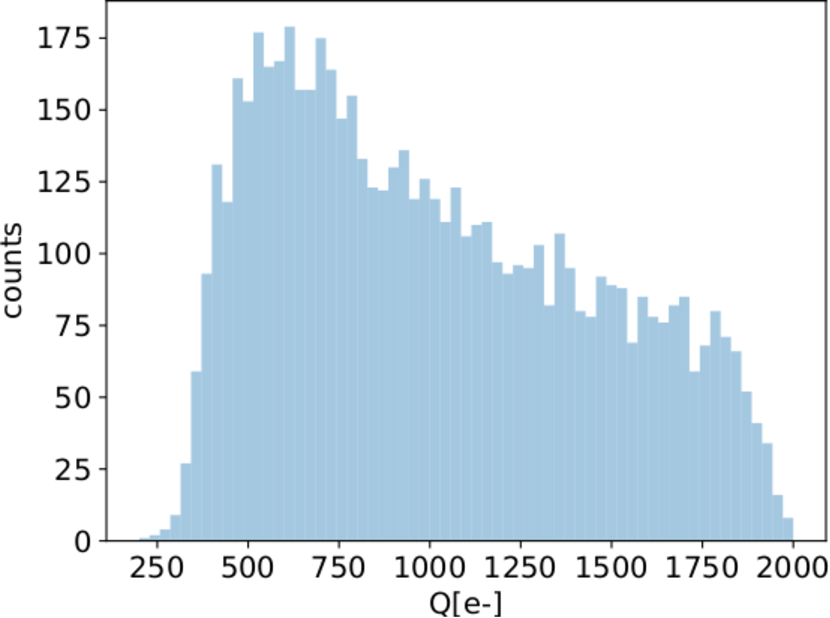
\includegraphics[width=.49\linewidth]{figures/test_beam/Q2_17_11.pdf}
        \end{figure}
        \begin{itemize}
            \item the collimators do not shield the detectors by all particles
            \item probably photons are produced by electrons in Al collimators
            \item for each accelerator pulse, 2 readout "cycle"  
        \end{itemize}
    \end{frame} 
    
    %%%%%%%%%%%%%%%%%%%%%%%%%%%%%%%%%%%%
    % Slide 3: <> %%
    %%%%%%%%%%%%%%%%%%%%%%%%%%%%%%%%%%%%
    \begin{frame}
        \frametitle{Test on beam: preliminary results}
        \begin{itemize}
            \item\textbf{Without} any collimator, DPP=\SI{0.04}{Gy}, t$_p$=\SI{4}{\us}, PRF=\SI{1}{Hz}
            \item MIP are expected to release \SI{2000}{\elementarycharge}$^-$, and because of rollorver are expected to be 300-400\si{\elementarycharge}$^-$
        \end{itemize}
        \medskip
        \begin{columns}
            \column{0.5\textwidth} 
                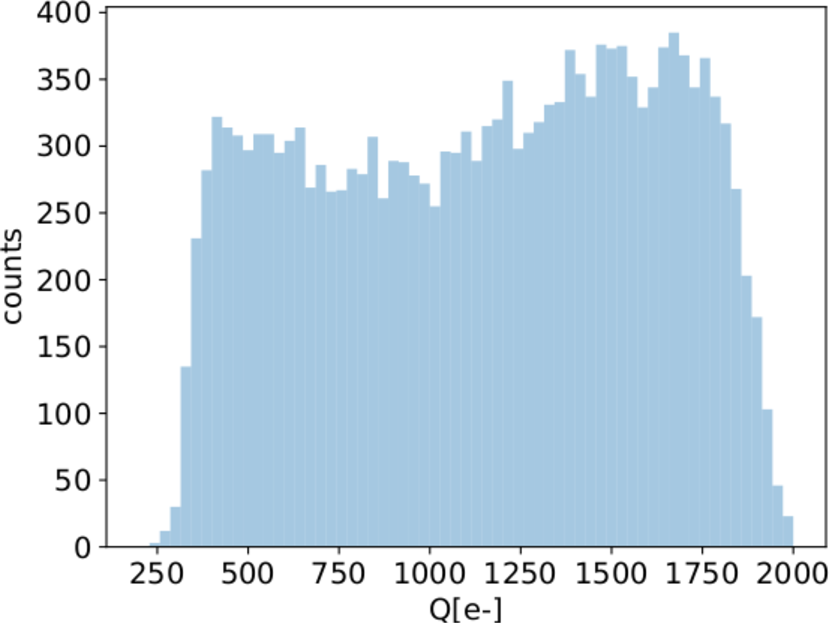
\includegraphics[width=1.1\linewidth]{figures/test_beam/Qe_17_32.pdf}
            \column{0.5\textwidth} 
                \begin{itemize}
                    \item ToT converted in charge
                    \item pixels turn on in N clock counts
                    \item after each pulse an induced signal on the whole matrix
                \end{itemize}
        \end{columns}   
        \medskip
        Need for a simulation to understand the data
    \end{frame}   